%----------------------------------------------------------------------------
\chapter{Irodalomkutatás}
\label{sec:LatexTools}
%----------------------------------------------------------------------------
\section{Létező megoldások keresése}
%----------------------------------------------------------------------------

Első lépésnek megpróbáltam már létező videó átméretező IP-ket keresni az interneten. Az Intel\cite{intelscaler}-nek és Xilinx\cite{xilinxscaler}-nek vannak már meglévő megoldásai, azonban ezek nem működnek mindig, sokszor hibásak, és van amit már nem is támogatnak. A két nagy gyártó saját scaler-jén kívül találtam harmadik féltől való megoldást is\cite{zipcores}, de ez is meglehetősen drága, úgyhogy egy saját IP kifejlesztésének igenis létjogosultsága van.

\section{Kép átméretezés}

Első lépésnek irodalomkutatást végeztem a képátméretezési technikákról. A képátméretezési technikák 2 fő csoportba oszthatóak: forward mapping és backward mapping.

\subsection{Forward mapping}

A forward mapping során egy bemeneti képnek a pixeleit próbáljuk közvetlenül átmappolni a kimeneti képnek a pixeleire. Ezt a \ref{pic:mapping} ábrán láthatjuk.  A kimeneti képen a képpontok ilyenkor nem fognak minden esetben pontosan ráesni egy-egy pixelre, ami miatt lyukak keletkezhetnek a kimeneti kép pixelei között. Erre egy lehetséges megoldás az, hogy az eredeti lép pixeleinek éleit vesszük, és ezt a formát átalakítjuk a kimeneti képre, majd ezután egy pixel értékét annak alapján állítjuk be, hogy az eredeti pixel értéke milyen mértékben van jelen ott. \cite{forwardmapping}

Ezek miatt belátható, hogy nem olyan szerencsés ezt a stratégiát használni. Sokkal jobb lenne, ha a kimeneti kép pixeleit mappolnánk át a bemeneti kép pixeleire, hiszen így biztosan minden kimeneti pixelre esne valamilyen érték. Ezt hívjuk backwards mappingnak.

\subsection{Backward mapping}

A backward mapping során fordítva, a kimeneti kép pixeleit feleltetjük meg a bemeneti kép pixeleihez. Ekkor ugyan szintén fenn áll a forward mapping során levő probléma, miszerint a pixelek nem fognak egy-egy pixelre ráesni a bemeneti képen, de ez itt nem probléma, hiszen itt minden pixel értékét ismerjük, tehát approximálhatjuk a nem egész koordinátán levő pixel értékét valamilyen algoritmus szerint. A \ref{pic:mapping} ábrán egy összehasonlítás látható a backward és forward mapping működése között.

\begin{figure}[!ht]
	\centering
	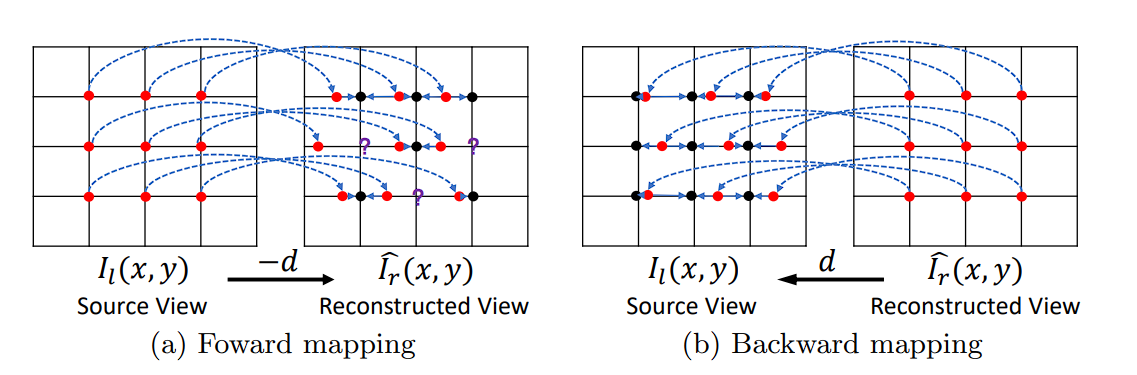
\includegraphics[width=120mm, keepaspectratio]{figures/mapping.png}
	\caption{A backward és forward mapping összehasonlítása \cite{forwardbackward}} 
	\label{pic:mapping}
\end{figure}

A projekt során a backward mapping megoldást használtam, hiszen ennek felhasználásával, könnyen lehet a kimeneti kép pixeleit a bemeneti képen való elhelyezkedésük alapján valamilyen algoritmus segítségével  meghatározni. Most tekintsünk meg néhány ilyen átméretező algoritmust.

\section{Bilinear filter}

A bilineáris szűrő az egyik egyszerűbb átméretezési technika. A lényege az, hogy a backward mapping során egy kimeneti pixelnek meghatározzuk a koordinátáját a bemeneti képen. Ez vagy ráesik egy pixelre, vagy nem. Ha nem esik rá egy pixelre teljesen, akkor viszont approximálni lehet az értékét a környező 4 pixel értékéből. A bilineáris interpoláció, mint a neve is mondja, 2 lineáris interpolációt végez el, vízszintesen, meg függőlegesen. A súlyok ilyenkor a környező pixelektől levő távolságok lesznek. Tehát egy 1D-s esetet nézve, ha a bal oldali pixelhez 2-szer olyan közel van a pixel mint a jobb oldalihoz, akkor a súlyok 0.66 és 0.33 lesznek. \cite{Wikipediabilinear_2024} A \ref{pic:bilinear} ábrán látható a vizualizációja az interpolációknak.

\begin{figure}[!ht]
	\centering
	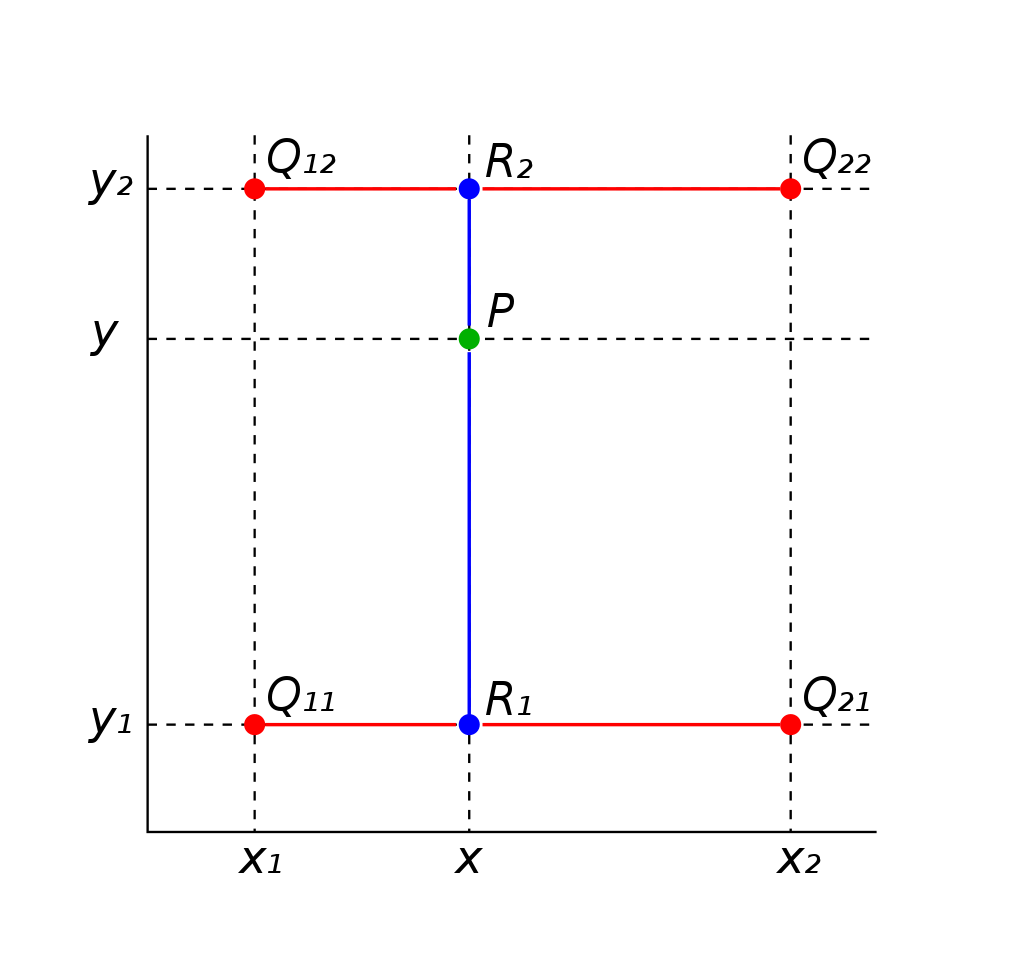
\includegraphics[width=100mm, keepaspectratio]{figures/bilinear.png}
	\caption{A bilineáris filter működése \cite{Wikipediabilinear_2024}} 
	\label{pic:bilinear}
\end{figure}
\newpage

A gyakorlatban 3 interpolációt kell megvalósítani, amiből a vízszintes irányban levő 2 interpolációt egyszerre, és utána pedig a függőleges interpolációt lehet elvégezni, ami már a kimenete lesz a filternek. A legegyszerűbb módon az alábbi képlettel lehet egy interpolációt elvégezni, mondjuk az alsó 2 pixelen:
\begin{equation}
	f(x,y_1) = \frac{x_2-x}{x_2-x_1}f(Q_{11}) + \frac{x-x_1}{x_2-x_1}f(Q_{21})
\end{equation}
Azonban azt látjuk, hogy ez a művelet osztást igényel, amit érdemes lenne elkerülni. Mivel biztosan tudjuk, hogy ez a 4 pixel szomszédos, emiatt a nevezőkben levő különbségek biztosan 1 lesznek. Az osztás tehát eltűnt. További egyszerűsítés, hogy az $x-x_1$ és a $x_2-x$ különbségeket könnyen tudjuk ábrázolni, hiszen a az $x-x_1$ az csak az $x$-nek az egész része, tehát ha fix pontosan ábrázoljuk a pixel koordinátáit, akkor csak a kettedes pont utáni biteket kell venni. Az $x_2-x$ pedig az előző számnak a komplementere, hiszen a kettő összege garantáltan 1. Így tehát ha meghatároztuk a kimeneti pixel koordinátáját a bemeneti képen, a bilineáris filterhez szükséges együtthatókat is könnyen meg tudjuk határozni. 

Innen már csak a szorzások vannak hátra, ami az előbb taglaltak miatt összesen 6 szorzás lesz, hiszen egy lineáris approximációhoz 2 szorzás kell. Ezek alapján az egyenletek a következőek lesznek:


\begin{align}		
	R_2 &= Q_{12} \left(X_2-X\right) + Q_{22} \left(X-X_1\right) \\
	R_1 &= Q_{11} \left(X-X_2\right) + Q_{21} \left(X-X_1\right)\\
	P &= R_2 \left(Y_1-Y\right) + R_1 \left(Y-Y_2\right)
	\label{eq:mult}
\end{align}

Ha ezt az algoritmust alkalmazzuk a kimeneti kép összes pixelére, akkor egy egész jó minőségű képet kaphatunk. Az algoritmus további előnye, hogy tetszőleges átméretezést tud megvalósítani, hiszen a kimeneti kép pixelei, csak a környező 4 pixeltől függ a bemeneti képen.

\subsection{Polyphase filter}

A polyphase filter, egy bonyolultabb szűrő architektúra, aminek a segítségével jobb minőségű képet tudunk generálni a bilineáris filterhez képest. A filter működése több dologban különbözik a bilineáris filtertől. 

Az első ilyen különbség, hogy a polyphase szűrő az nem a környező 4 pixel értékéből dolgozik, hanem tetszőleges mennyiségű körrnyező sort/oszlopot tud felhasználni a kimeneti pixel értékének meghatározásához. A bilineáris filternél 2 sort és 2 oszlopot használtunk, tehát mint vertikális, mind horizontális irányban 2-2 "tap" je van a bilineáris szűrőnek. A polyphase filter-t sok esetben 4 vertikális és 4 horizontális tap-el alkalmazzák, tehát horizontális és vertikális irányban is 4-4 pixelt, azaz a környező 16 pixelt veszik figyelembe a kimenet meghatározásához. 

A második fontos különbség az az együtthatók előállítása. A bilineáris filternél a kimeneti pixel közvetlen helyzetéből van meghatározva a környező 4 pixel súlya az alapján, hogy milyen távol van a pixel ezektől. A polyphase szűrőnél ezzel ellentétben előre le vannak generálva az együtthatók, valamilyen algoritmus alapján. Ez az algoritmus általában a bemeneti és kimeneti kép arányszámát használja fel együttható generálásra. A Xilinx ajánlása alapján \cite{Xilinx_poly} (48 oldal) az úgynevezett Lánczos algoritmus segítségével lehet  előállítani ilyen együtthatókat.

Ezen kívül fontos megjegyezni, hogy az algoritmus nem csak (4x4 tap esetén) említett 16 algoritmust használja. Ugyanis ahogy a szűrő neve mondja, a kimeneti pixel bemeneti képen elhelyezkedő képpont "fázisa" alapján válsztja ki a megfelelő együtthatókat. Nézzük meg egy egyszerű példán a működést, 1 dimenzióban az egyszerűség kedvéért. Tegyük fel, hogy a bemeneti sorban 6 pixel van, és a kimeneti sorban pedig 5. Ekkor ha megfeleltetjük a kimeneti pixeleket a bemeneti képen, akkor az \ref{pic:poly_1d} ábrát fogjuk kapni ("O"-kimeneti pixel pixel, "X" bemeneti pixel)

\begin{figure}[!ht]
	\centering
	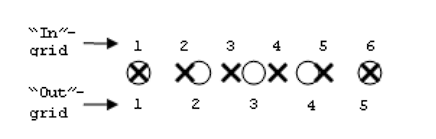
\includegraphics[width=100mm, keepaspectratio]{figures/poly_1d.png}
	\caption{A polyphase filter működése, 1 dimenzióban \cite{Xilinx_poly}} 
	\label{pic:poly_1d}
\end{figure}

Mint látjuk, a kimeneti pixel 4 féle fázisban lehet. Ezek a fázisok $0$, $1/4$, $2/4$, $3/4$. Ezeket úgy kaptuk meg hogy elosztottuk a kimeneti és bemeneti kép méretét (technikailag a kimenet-1 és a bemenet-1 méreteket), mellyel $5/4$ -et kaptunk, majd ezt mindig hozzáadtuk az előző pixel értékéhez, és így megkaptuk a kimeneti pixelek koordinátáit, a bemeneti képen: $0, 5/4, 10/4, 15/4, 20/4$, melyekből már látszanak az előbb megállapított fázisok. Ekkor tehát szűrő az alapján, hogy milyen fázisban van, más együtthatókat használ a környező pixelek súlyozására. Éppen ezért a polyphase szűrő nem együtthatókkal, hanem úgynevezett coefficient bank-al rendelkezik.

\subsection{Separable filter}

A polyphase szűrő egyszerűbb, és erőforrás takarékosabb megvalósításához érdemes a separable, vagyis úgynevezett szétválasztható szűrők fogalmának ismertetése. Ez csupán annyit takar, hogy pl a bilineáris szűrő megvalósításához hasonlóan, a szűrőnket szétdaraboljuk több, 1 dimenziós interpolációra. Ez a polyphase szűrőnél azt fogja jelenteni, hogyha pl 4-4 tap-es szűrőről van szó, akkor először a 4 oszlopon hajtunk végre egy interpolálást, amiből kapunk 4 értéket, majd végül ezen 4 értéken vízszíntes irányban hajtunk végre egy interpolálást, ezzel egyszerűsítve a filter architektúráját.\cite{Bart Wronski_2020} Ezt a mőködést a \ref{poly_2d} ábra szemlélteti.

\begin{figure}[!ht]
	\centering
	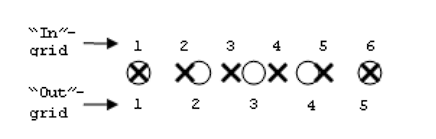
\includegraphics[width=100mm, keepaspectratio]{figures/poly_1d.png}
	\caption{Egy separable polyphase filter működése} 
	\label{pic:poly_2d}
\end{figure}

Fontos megjegyezni, hogy nem minden polyphase filter szétválasztható, ez csak akkor teljesül, ha olyan együtthatókat generálunk, amelyek erre képesek.

